\problemname{Mancala}

\begin{figure}[p]
    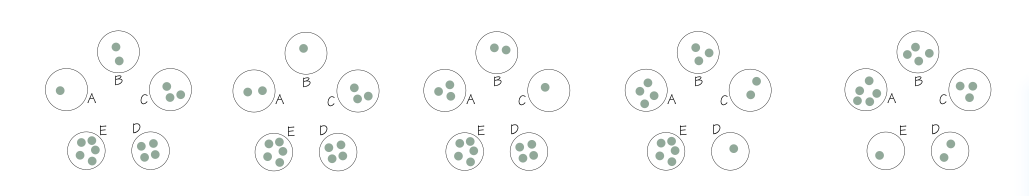
\includegraphics{figur.png}
	\caption{Exempelfall 1}
\end{figure}

\emph{Mancala} är ett urgammalt spel från Afrika, från vilket vi lånar principerna i denna uppgift. Figuren ovan visar 5 ställningar. I varje ställning ser vi 5 \emph{skålar} i vilka ligger ett varierat antal \emph{frön}. Längst till vänster ser vi exempel på en \emph{utgångsställning} och längst till höger exempel på en önskad \emph{slutställning}. För att nå slutställningen behöver 4 drag göras.

Ett drag består av följande delar:
\begin{enumerate}
	\item Välj ut en skål och ta upp samtliga frön som finns i den.
	\item Välj en riktning, \emph{medurs} eller \emph{moturs}.
	\item \emph{Så} först ett frö i den skål du just tömde. Så sedan ett frö i varje skål, utefter den riktning du valde, så långt de räcker.
\end{enumerate}

Upprepa sedan punkterna 1-3 tills önskad slutställning uppnås.

I exemplet i figuren utförs följande drag: Först väljer vi skål B och sår i riktning moturs. I nästa drag väljer vi skål C och sår återigen moturs. I tredje draget väljer vi skål D och riktning moturs. I fjärde och sista draget hämtar vi fröna från skål E. Nu kan vi välja vilken riktning vi fill, resultatet blir ändå det samma. Därmed har vi från utgångsställningen 1, 2, 3, 4, 5 nått slutställningen 5, 4, 3, 2, 1 på fyra drag (skålarnas innehåll presenteras i ordningen A, B, C, D, E).

Skriv ett program som tar emot en utgångsställning och en slutställning och som tar reda på det minsta antalet drag som krävs för att nå målet. I våra tester kommer det aldrig att behövas fler än 6 drag.

Det största antalet frön i en skål i utgångsställningen är 10.

\section*{Indata}
Indata består av två rader. Den första raden innehåller utgångsställningen som 5 blankstegs-separerade heltal med antalet frön i skålarna (i ordningen A, B, C, D, E). Den andra raden innehåller slutställningen, presenterad på samma sätt. Ingen skål innehåller fler än 10 frön.

\section*{Utdata}
Skriv ut ett heltal: det minsta antalet drag som behövs för att uppnå slutställningen.

\section*{Poängsättning}
Din lösning kommer att testas på flera testfall. För att få 100 poäng så måste du klara alla testfall.

